\documentclass[aspectratio=1610]{beamer}
\usepackage[utf8]{inputenc}
\usepackage[T1]{fontenc}
\usepackage{graphicx}
\usepackage{grffile}
\usepackage{longtable}
\usepackage{wrapfig}
\usepackage{rotating}
\usepackage[normalem]{ulem}
\usepackage{amsmath}
\usepackage{textcomp}
\usepackage{amssymb}
\usepackage{capt-of}
\usepackage{hyperref}
\usepackage{svg}
\usetheme{Frankfurt}
\usecolortheme{seagull}
\usefonttheme{}
\useinnertheme{}
\useoutertheme{}
\author{\href{mailto:denis.holub@stud.sbg.ac.at}{Denis Holub}, \href{mailto:fabian.nedoluha@stud.sbg.ac.at}{Fabian Nedoluha}}
\date{October 17, 2019}
\title{Quantencomputing \& DNA-Computing}
\institute[INST]{\href{https://www.uni-salzburg.at/index.php?id=39957}{Univ. Salzburg - Computerwissenschaften}}
\AtBeginSection[]{\begin{frame}<beamer>\frametitle{Agenda}\tableofcontents[currentsection]\end{frame}}
\hypersetup{
 pdfauthor={\href{mailto:denis.holub@stud.sbg.ac.at}{Denis Holub}, \href{mailto:fabian.nedoluha@stud.sbg.ac.at}{Fabian Nedoluha}},
 pdftitle={Quantencomputing \& DNA-Computing},
 pdfkeywords={Quantencomputing DNA-Computing RNA-Computing},
 pdfsubject={Eine Einführung in die Welt der Quanten- und DNA-Computer.},
 pdflang={Germanb}}
\begin{document}

\maketitle

\section{Quantencomputing}
\label{sec:orgb98938d}

\subsection{Bit vs. Qubit}
\label{sec:org4210bed}

\begin{frame}[label={sec:orgb561d02}]{Bit vs. Qubit}
\begin{itemize}
\item Binärsystem
\item Bit – 0/1
\item Qubit – 0/1/Superposition von beiden
\item Angeregter Zustand von Elektron, Photon Polarisation
\end{itemize}

\begin{equation}
    |\psi\rangle = a \, |0\rangle + b \, |1\rangle
\end{equation}
\end{frame}

\begin{frame}[label={sec:org68a03d4}]{Bit vs. Qubit}
\begin{itemize}
\item Bits – 1 Zustand des Computers
\item Qubit – Mehrere Zustände gleichzeitig
\item Qubit – 2\(^{\text{n}}\) Möglichkeiten
\end{itemize}
\end{frame}

\subsection{Quanten Computing}
\label{sec:orgb13c2b2}

\begin{frame}[label={sec:org4854eea}]{Quanten Computing}
\begin{itemize}
\item Mehrere Zustände -> parallel rechnen
\item Verbinden von Qubits
\item Probleme mit dem Messen
\item Fehlerrate
\item 0,015 Kelvin -> Supraleiter
\item D-Wave behauptet 2048 verbundene Qubits -> kein Quantum Computing
\end{itemize}

\begin{center}
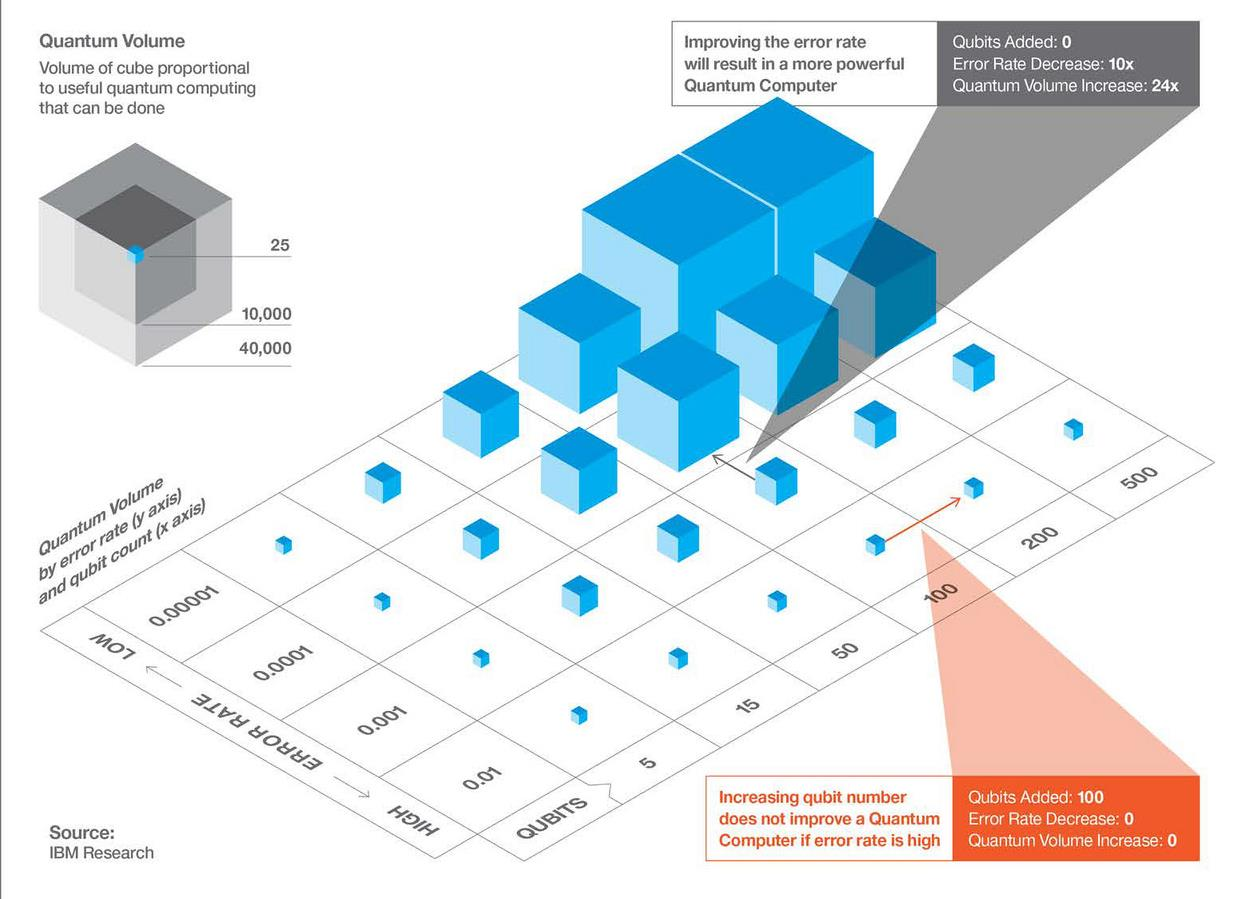
\includegraphics[width=0.4\textwidth]{./image-000.jpg}
\end{center}
\end{frame}

\subsection{Geschichte}
\label{sec:org4a63630}

\begin{frame}[label={sec:org8e5df60}]{Geschichte – Quantum Computers}
\begin{itemize}
\item 2016
\begin{itemize}
\item IBM 5 Qubits
\end{itemize}
\item Anfang 2017
\begin{itemize}
\item IBM und Intel haben 17 verbundene Qubits
\item IBM verkauft Quantum Computer an NASA und Google
\end{itemize}
\item September 2017
\begin{itemize}
\item Größte Molekule Simulation Beryllium Hybride (BeH2)
\end{itemize}
\item 2018
\begin{itemize}
\item Google 72 Qubits
\item Intel 49 Qubits
\end{itemize}
\item 2019
\begin{itemize}
\item IBM Q System ONE (20 Qubits) – kommerziel verkauft
\item IBM Im September 53 Qubits
\item Google 53 Qubits
\end{itemize}
\end{itemize}
\end{frame}

\subsection{IBM Q System ONE (20 Qubits)}
\label{sec:orgb5f2e06}

\begin{frame}[label={sec:orge905aec}]{IBM Q System ONE (20 Qubits)}
\begin{figure}[htbp]
\centering
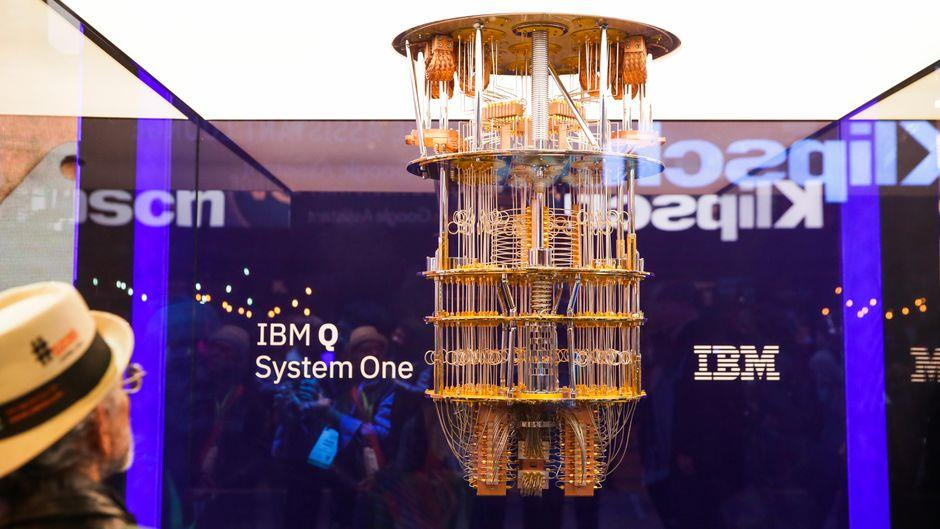
\includegraphics[height=0.7\textheight]{./image-001.jpg}
\caption{\url{https://www.cnet.com}}
\end{figure}
\end{frame}

\subsection{Computing}
\label{sec:orgfd4c051}

\begin{frame}[label={sec:org4e77e77}]{Computing}
\begin{figure}[htbp]
\centering
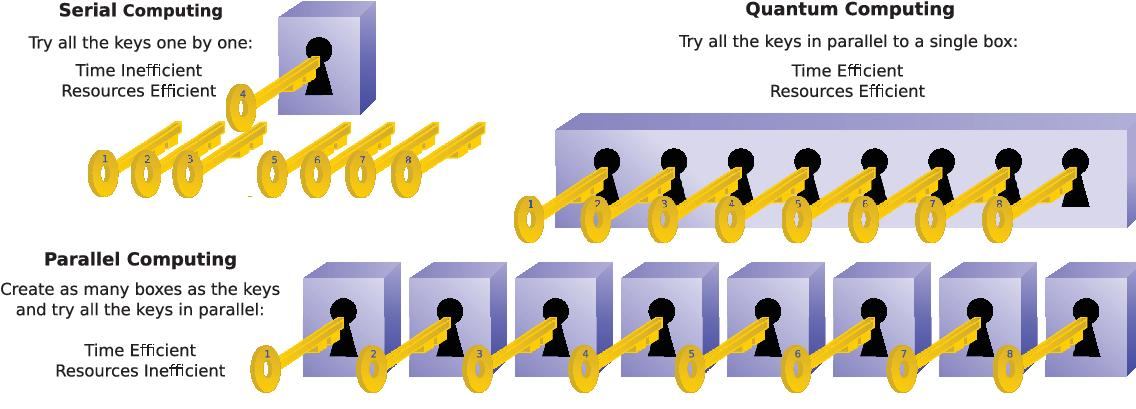
\includegraphics[height=0.5\textheight]{./image-002.jpg}
\caption{\url{https://www.semanticscholar.org}}
\end{figure}
\end{frame}

\subsection{Quantum Algorithmen}
\label{sec:org8e87eb7}
\begin{frame}[label={sec:org2bbb0c8}]{Quantum Algorithmen}
\begin{itemize}
\item Faktorisierung ganzer Zahlen -> RSA Verschlüsselung
\item Algorithmen für normalen Rechner
\begin{itemize}
\item O((log N)\(^{\text{3}}\))
\end{itemize}
\item Shor´s Algorithmus (1994) für Quantum Computer
\begin{itemize}
\item O((log n)\(^{\text{2}}\) (log log n) (log log log n))
\end{itemize}
\end{itemize}
\end{frame}

\section{DNA-Computing}
\label{sec:orge9ae4bd}

\subsection{Einführung}
\label{sec:org6ce5334}
\begin{frame}[label={sec:org5b9834d}]{Biocomputer}
\begin{itemize}
\item Biochemische Computer
\item Biomechanische Computer
\item Bioelektronische Computer
\end{itemize}
\end{frame}

\begin{frame}[label={sec:org62fba69}]{DNA Computing}
\begin{itemize}
\item Verarbeiten von Daten mit Hilfe von biologischen Systemen
\item DNA kann zum Programmieren verwendet werden
\item Parallelismus (jeder DNA Strang ist ein Prozessor)
\item Molekulare Größen (10\(^{\text{-9}}\) m)
\end{itemize}
\end{frame}

\begin{frame}[label={sec:orgb74b855}]{Desoxyribonukleisäure und Ribonukleisäure}
\begin{figure}[htbp]
\centering
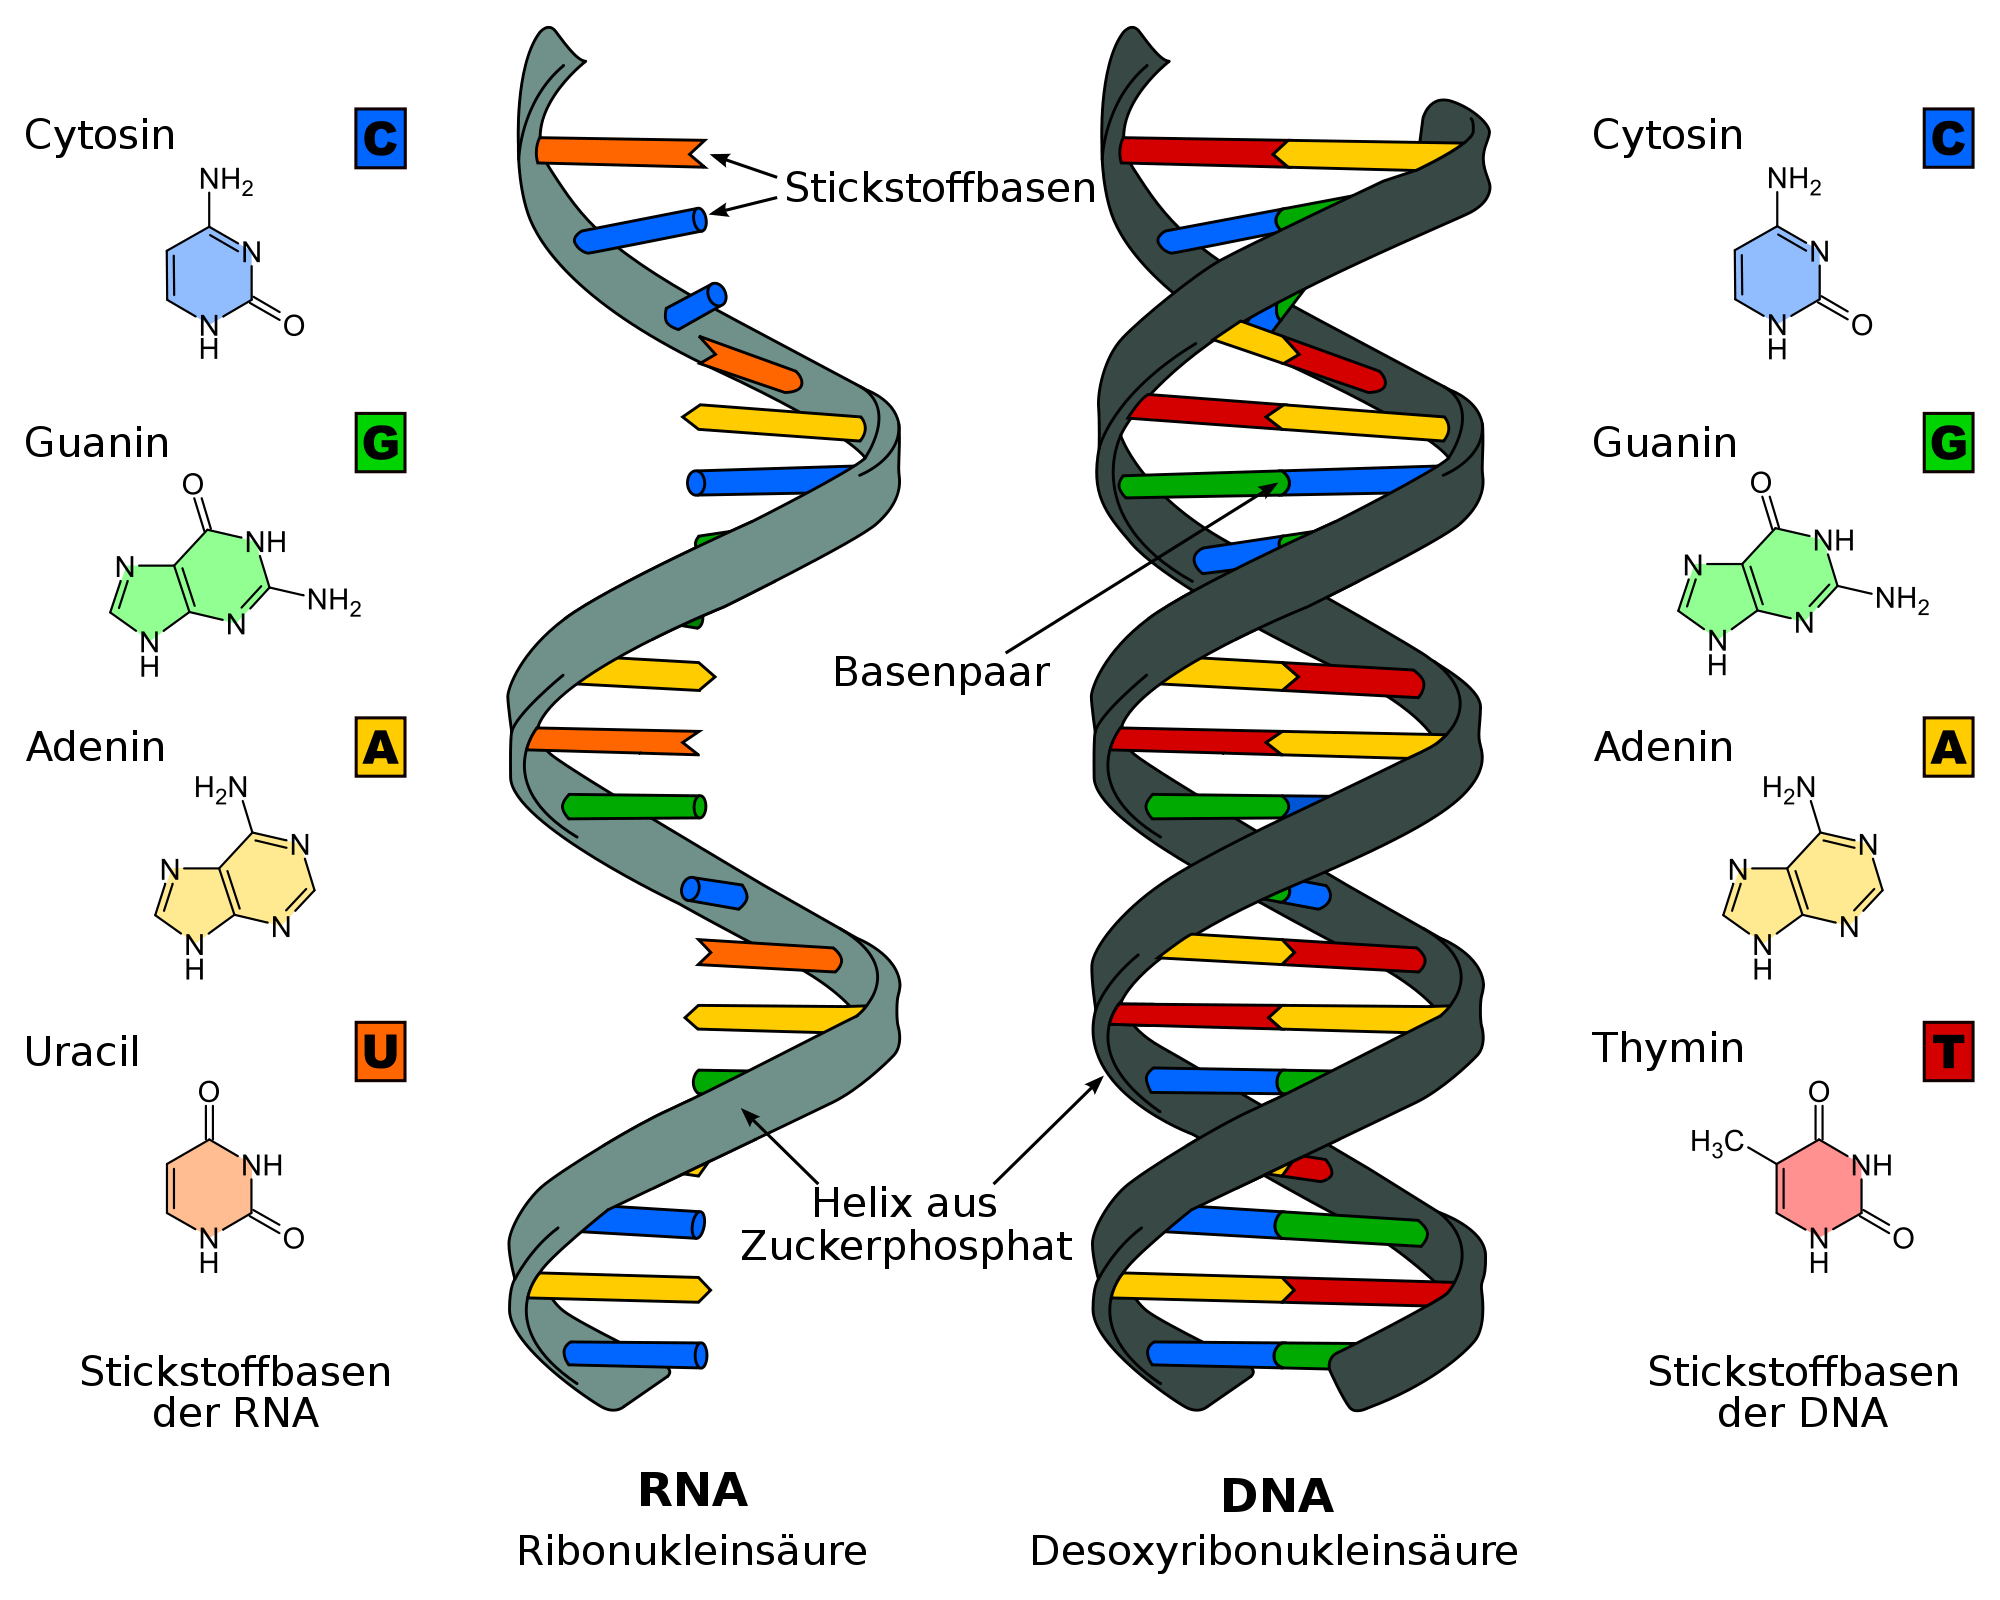
\includegraphics[height=0.7\textheight]{./2000px-Difference_DNA_RNA-DE.svg.png}
\caption{\url{https://commons.wikimedia.org/wiki/File:Difference\_DNA\_RNA-DE.svg}}
\end{figure}
\end{frame}

\begin{frame}[label={sec:orgbc9ec26}]{Basisoperationen}
\begin{block}{Manipulation anhand von Enzymen}
\begin{itemize}
\item Polymerasen (verlängern)
\item Nukleasen (aufschneiden)
\item Ligasen (verbinden)
\end{itemize}
\end{block}

\begin{block}{Vervielfältigung}
Dank der Polymerase-Kettenreaktion (PCR)\footnote{Kary Mullis (1985)} kann DNA recht einfach kopiert werden.
\end{block}
\end{frame}

\subsection{Meilensteine}
\label{sec:orgcab4414}

\begin{frame}[label={sec:org2bbea22}]{Meilensteine}
\begin{itemize}
\item 1950er Richard Feynman: Erste Ideen
\item 1994 Adleman löst Hamiltonkreisproblem mit DNA
\item 1999 William Ditto baute einen organischen Computer mit Blutegel Neuronen
\item 2012 Harvard enkodiert ein Buch mit 55.000 Wörtern in DNA
\item 2013 Stanford entwickelt ersten biologischen Transistor "Transcriptor"
\item 2017 Cornell Implemented a non-deterministic universal Turing machine using DNA
\item 2017 Yaniv Erlich und Dina Zielinski entwickeln Kodierungssystem welches das Speichern von 215 Petabyte in 1 Gram DNA ermöglicht
\end{itemize}
\end{frame}

\subsection{DNA als Computation Maschine}
\label{sec:org601d033}

\begin{frame}[label={sec:org79fdf56}]{DNA als Computation Maschine}
\begin{itemize}
\item Derzeit eher theoretischer Natur
\item Eignet sich gut für viele kleine Probleme
\item Reduzierte Rechenzeit (Parallelismus)
\item Dynamische Programmierung
\end{itemize}
\end{frame}

\subsection{Hilfsmittel}
\label{sec:org034f50a}

\begin{frame}[label={sec:org337e70a}]{Hilfsmittel}
\begin{itemize}
\item Simulations Software für Genome und Moleküle
\item Drucker
\item Lesegeräte
\end{itemize}
\end{frame}

\subsection{Wissenschaftliche Papers}
\label{sec:org67ba790}
\begin{frame}[label={sec:orgd408b33}]{Wissenschaftliche Papers}
\begin{itemize}
\item DNA computation: Theory, practice and prospects (1998)
\item Toward molecular programming with DNA (2008)
\item The DNA query language DNAQL (2013)
\item High capacity data hiding method in DNA with mutation handling (2014)
\item A dual security scheme using DNA key based DNA cryptography (2014)
\item A secure image based authentication schme employing DNA crypto and steganography (2015)
\item Analog and digital memory in living cells (2017)
\item A DNA-based archival storage system (2016)
\end{itemize}
\end{frame}

\subsection*{Vielen Dank}
\label{sec:org6cf500d}
\begin{frame}[label={sec:orgcc7bb64}]{Das Ende}
Vielen Dank für Ihre Aufmerksamkeit
\end{frame}
\end{document}
